\documentclass[revision-guide.tex]{subfiles}
%% Current Author: PS
\setcounter{chapter}{0}
\begin{document}
\chapter{Mechanics}
\begin{content}
\item scalars and vectors
\item moment of a force
\item kinematics
\item Newton’s laws of motion
\item conservation of linear momentum
\item density
\item pressure
\end{content}

\section*{Candidates should be able to:}

\section{Scalars and Vectors}
\spec{distinguish between scalar and vector quantities and give examples of each}
A scalar quantity\footnote{strictly we are modelling a physical quantity as a mathematical object} is one which has only a magnitude whereas a vector has \emph{both} magnitude and direction. We often use positive and negative values to indicate direction (e.g. $v=-2\ ms^{-1}$) but this does not mean that all negative values are vectors!

Note that there are different ways of multiplying vectors and scalars. Two vectors can be multiplied to give a scalar \emph{or} a vector. For example, work done is the (scalar) product of force and displacement, both vectors.

\spec{resolve a vector into two components at right angles to each other by drawing and by calculation}

Vectors can be split into two components using trigonometry. The diagram below shows a velocity vector being split into horizontal and vertical components $v_x$ and $v_y$.

\begin{figure}[h]
\begin{center}
\begin{tikzpicture}
	\draw[very thick, black, ->] (0,0) -- node[above] {$\mathbf{v}$}  (5,2.5);
	\draw[very thick, purple, ->] (0,0) -- node[below] {$\mathbf{v_x}$} (5,0);
	\draw[very thick, purple, ->] (0,0) -- node[left]{$\mathbf{v_y}$}(0,2.5);
	\draw [very thick,gray](1,0) arc (0:26.6:1);
	\draw [gray](1,0.25) node[right]{$\theta$};
	\draw (7,1.25) node[right] {
		$\begin{aligned}
		\mathbf{v}&=\mathbf{v_x + v_y}\\
		v_x &= v\cos{\theta}\\
		v_y &= v\sin{\theta}
		\end{aligned}$};
\end{tikzpicture}
\end{center}
\end{figure}

\spec{combine any number of coplanar vectors at any angle to each other by drawing}

Vectors can be added by placing them end to end. The resultant vector is the one joining the start of the first vector to the end of the final vector. Its magnitude and direction can be calculated by trigonometry or scale drawing.

\begin{figure}[h]
	\begin{center}
	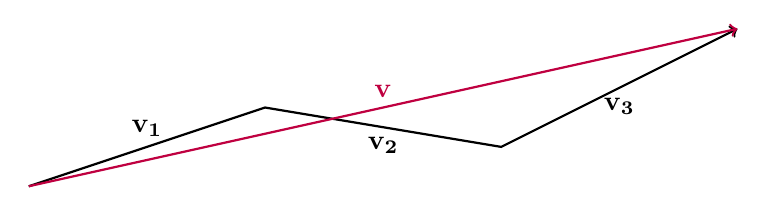
\begin{tikzpicture}
	\draw[thick,->] (0,0) -- node[above] {$\mathbf{v_1}$} (3,1) -- node[below] {$\mathbf{v_2}$} (6,.5) -- node[below] {$\mathbf{v_3}$} (9,2);
	\draw[thick,purple,->] (0,0) -- node[above]{$\mathbf{v}$} (9,2);
	\end{tikzpicture}
	$$\mathbf{v} = \mathbf{v_1}+\mathbf{v_2}+\mathbf{v_3}$$
	\end{center}
\end{figure}

\section{Static Equillibrium}

\spec{calculate the moment of a force and use the conditions for equilibrium to solve problems (restricted to
	coplanar forces)}

The moment of a force is calculated by multiplying its magnitude by the perpendicular distance of the force's line of action to the pivot point. This is mathematically equivalent to multiplying the distance from the pivot by the component of the force perpendicular to that distance.

\begin{figure}[h]
	\centering
	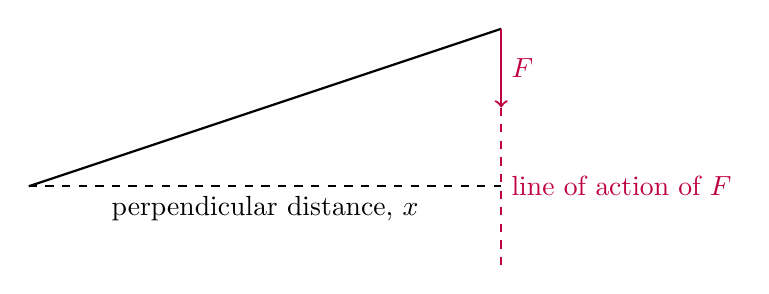
\begin{tikzpicture}
		\draw[thick] (0,0) -- (6,2);
		\draw[thick, purple, ->] (6,2) -- node[right]{$ F$}(6,1);
		\draw[thick, purple, dashed] (6,1) -- node[right] {line of action of $F$}(6,-1) ;
		\draw[thick, dashed] (0,0) -- node[below]{perpendicular distance, $x$} (6,0);

	\end{tikzpicture}
	$$\mathrm{moment} = Fx $$
\end{figure}

The conditions for equilibrium are:
\begin{enumerate}
	\item The sum of all the forces acting on the object must be zero.
	\item The sum of all the moments on an object must be zero.
\end{enumerate}
\begin{example}
	A Tower Crane lifts a load into position. The load has a weight of \SI{4.0e4}{N} and the arm of the crane has a weight of \SI{1.2e5}{N}.

	Calculate the required weight of the counterweight and the force the tower must support. Assume the centre of mass of the arm is at its centre.

	\vspace{1cm}

		\begin{center}
		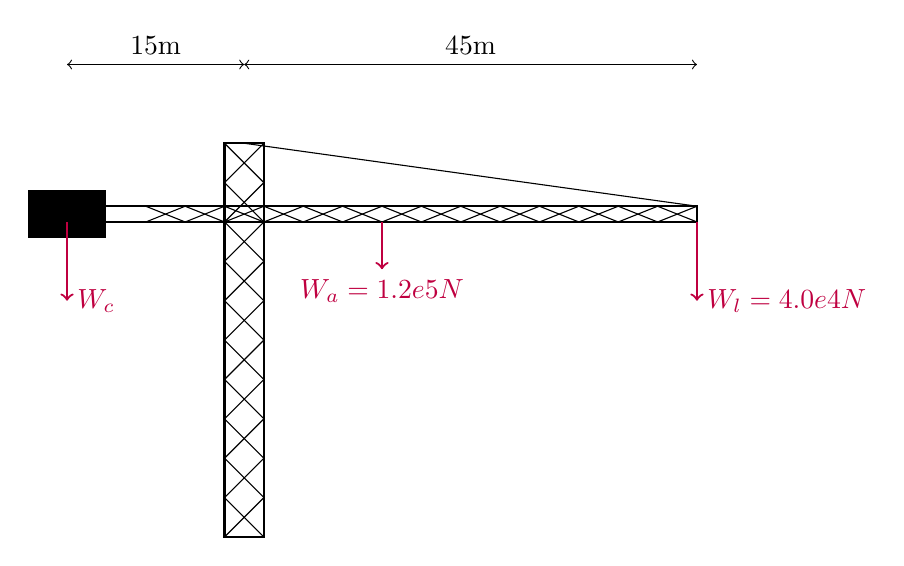
\begin{tikzpicture}
					\draw[thick] (2,0) rectangle (2.5,5);
					\draw[thick] (0,4) rectangle (8,4.2);
					\fill (-0.5,3.8) rectangle (.5,4.4);
					\draw(2.25,5) -- (8,4.2);
					\foreach \x in {0,1,...,13} {
						\draw (1+0.5*\x,4) -- (1.5+0.5*\x,4.2);
						\draw (1+0.5*\x,4.2) -- (1.5+0.5*\x,4);
					}
					\foreach \y in {0,1,...,9} {
						\draw (2,0+0.5*\y) -- (2.5,0.5+0.5*\y);
						\draw (2.5,0+0.5*\y) -- (2,0.5+0.5*\y);
					}
					\draw[purple, thick, ->] (8,4) -- (8,3) node[right]{$W_l=\SI{4.0e4}{N}$};
					\draw[purple, thick, ->] (4,4) -- (4,3.4) node[below]{$W_a=\SI{1.2e5}{N}$};
					\draw[purple,thick, ->] (0,4) -- (0,3) node[right]{$W_c$};
					\draw[<->] (0,6) -- node[above]{15m}(2.25,6);
					\draw[<->] (2.25,6) -- node[above]{45m}(8,6);
				\end{tikzpicture}
		\end{center}

		\textbf{Answer}

		We begin by taking moments around the tower of the crane. The weight of the arm, $W_a$, acts \SI{15}{m} from the tower so solving for moments gives:

		$$ 15W_c = 15W_a + 25W_l $$
		$$ W_c = \SI{4.2e5}{N} $$

		The sum of the downward forces must equal the reaction force of the tower so:

		$$ R = \SI{4.0e5}{N} $$
\end{example}

\section{Kinematics}

\spec{construct displacement-time and velocity-time graphs for uniformly accelerated motion}

For uniform acceleration, a graph of velocity against time will be linear, with the formula $ v=u+at$, and a graph of displacement against time will be parabolic, with the formula $s=ut+\frac{1}{2}at^2$.

\begin{center}
	\begin{tikzpicture}[domain=0:3]
		\draw[thick,->] (0,0) -- (3,0) node[below]{$t$};
		\draw[thick,->] (0,0) -- (0,3) node[left]{$s$};
		\draw[thick,->] (4,0) -- (7,0) node[below]{$t$};
		\draw[thick,->] (4,0) -- (4,3) node[left]{$v$};
		\draw[color=purple] plot (\x+4,{.2+0.4*\x});
		\draw[color=purple] plot (\x,{.2*\x+0.2*\x^2});
	\end{tikzpicture}
\end{center}

\spec{identify and use the physical quantities derived from the gradients of displacement--time and areas and gradients of velocity--time graphs, including cases of non-uniform acceleration}

The quantities are given in the table below:

\begin{tabular}{r|ll}
	& gradient & area  \\ \hline
	displacement-time & velocity & -- \\
	velocity-time & acceleration & displacement \\
\end{tabular}

If the graph is non-linear then the gradient of a tangent must be taken. Note that areas below the axis in a velocity-time graph represent \emph{negative} displacement.

\spec{recall and use:}
\begin{align*}
	v &= \frac{\Delta x}{\Delta t}\\
	a &= \frac{\Delta v}{\Delta t}
\end{align*}

\spec{recognise and use the kinematic equations for motion in one dimension with constant acceleration:}
\begin{align*}
	s &= ut + \frac{1}{2}at^2 \\
	v^2 &= u^2 + 2as \\ s &= \left( \frac{u+v}{2} \right) t
\end{align*}

\spec{recognise and make use of the independence of vertical and horizontal motion of a projectile moving freely under gravity}

When an object moves in a uniform gravitational field it motion can be modeled by considering the horizontal and vertical components of motion separately. The horizontal component has a constant velocity and the vertical has a constant acceleration.

\begin{example}
A ball is thrown with a velocity of \SI{5}{m.s^{-1}} from a height of \SI{1.2}{m}. If its initial angle to the horizontal is \ang{50} calculate the distance it travels before it hits the ground.
\answer

The first step is to split the velocity into horizontal and vertical components:
	\begin{align*}
		v_x = 5\cos{50}\\
		v_y = 5\sin{50}
	\end{align*}

	The time for the ball to reach the ground can now be calculated using the vertical motion and the equation $s=ut+\frac{1}{2}at^2$, setting $s = \SI{-1.2}{m}$. This gives $t=\SI{1.02}{s}$.

	Finally, the horizontal distance is calculated using the simple constant velocity formula to give $x=\SI{3.28}{m}$.
\end{example}

\section{Forces}

\spec{recognise that internal forces on a collection of objects sum to zero vectorially}

This is as a result of Newton's Third Law.

\spec{recall and interpret statements of Newton’s laws of motion}
\begin{enumerate}
	\item An object will remain at rest, or continue at a constant velocity, unless a resultant force acts upon it.
	\item $F=ma$, where $F$ is the vector sum of the forces acting on the body. Or, alternatively $F=\frac{dp}{dt}$ (see below).
	\item For every force of object A acting on object B there exists a force of the same type, of equal magnitude and opposite direction of object B acting on object A.

	\emph{It is important to be able to distinguish the `equal and opposite' forces which may act on a single object in equilibrium from a Newton's Third Law pair of forces.}
\end{enumerate}

\spec{recall and use $F = ma$ in situations where mass is constant}

Remember that $F$ is the \emph{resultant} force acting on the body.

\spec{understand the effect of kinetic friction and static friction}

\spec{use $F_k = \mu_k N$ and $F_s = \mu_s N$, where $N$ is the normal contact force and $\mu_k$ and $\mu_s$ are the coefficients of kinetic friction and static friction, respectively}

Friction occurs between two objects when they are pushed together by a normal force. A useful model is that the maximum size of the frictional force is proportional to the normal force. There is usually a difference between the constant of proportionality when the two surfaces are stationary compared to each other (static friction) compared to when they are sliding past each other (kinetic friction). It is usually the case that $\mu_k < \mu_s$.

An interesting result is that blocks of different masses should take the same distance to slide to a halt:

\[ s = \frac{\frac{1}{2}mv^2}{F} = \frac{\frac{1}{2}mv^2}{\mu_k N} = \frac{\frac{1}{2}mv^2}{\mu_k mg} = \frac{v^2}{2\mu_k g} \]

\spec{recall and use the independent effects of perpendicular components of a force}

As with velocities, forces can be split into two perpendicular components and their effects considered independently.

\begin{example}
A block of mass \SI{4}{kg} is on a frictionless slope of \ang{30}. Calculate the rate at which it accelerates down the slope.

\begin{tikzpicture}
	\draw[thick] (0,0) -- (10,0);
	\draw[thick] (0,0) -- (10,5.77);
	% TODO
\end{tikzpicture}

\answer

The weight should be split into components along the slope and perpendicular to the slope (shown in green). Only the component along the slope contributes to the acceleration.

\[ a = \frac{F}{m} = \frac{mg\cos{30}}{m} = \SI{8.5}{ms^{-2}} \]

This question could be extended to include friction by calculating the normal force, the frictional force and hence a new acceleration. If $\mu_k = 0.4$ then the answers are \SI{19.62}{N}, \SI{7.85}{N} and \SI{6.5}{ms^{-2}} respectively (Try it!)

\end{example}

\spec{recall and use p = mv and apply the principle of conservation of linear momentum to problems in one dimension}

Momentum is a conserved quantity (along with energy and charge). It can be calculated using the formula $p=mv$ where $p$ is the momentum. In any closed system the total momentum of the particules must remain constant. This can be used to predict the outcomes of collisions in certain cases.

\spec{distinguish between elastic and inelastic collisions}

An elastic collision is one in which \emph{kinetic energy} is conserved. An inelastic collision is one in which it is not. In general, a collision in which two objects adhere will not conserve kinetic energy as the final velocity will be given by:
$$ v = \frac{m_1u_1+m_2u_2}{m_1+m_2} $$
and therefore the final kinetic energy will be given by:
\[ \text{KE} = \frac{1}{2}(m_1+m_2)v^2 = \frac{1}{2}\frac{\left( m_1u_1+m_2u_2\right)^2}{m_1+m_2}\]
which cannot be equal to the original kinetic energy.

\spec{relate resultant force to rate of change of momentum in situations where mass is constant and recall and use $F = \frac{\Delta P}{\Delta t}$}

Newton's second law is more properly given by:

\[ F = \frac{dp}{dt} \]

This simplifies to the GCSE formulation for constant mass:

\[ F = \frac{dp}{dt} = m\frac{dv}{dt} = ma \]

A simplified version is:
$$F = \frac{\Delta P}{\Delta t}$$

This will give the correct result for a constant force or otherwise give the average force.

\spec{recall and use the relationship impulse = change in momentum}

Multiplying both sides of the equation above by time gives:
$$ F \Delta t = \Delta P $$

The quantity on the left hand side is the impulse.

\spec{recall and use the fact that the area under a force-time graph is equal to the impulse}

Using calculus to solve differential version of Newton's Second Law above gives:
$$ \Delta P = \int_{t_0}^{t_1} F dt $$
The right-hand side of this equation represents the area under a force-time graph.

\spec{apply the principle of conservation of linear momentum to problems in two dimensions}

When objects are free to move in two dimensions then momentum must be conserved along two axis.

\begin{example}
	Two objects are able to slide frictionlessly over a horizontal surface. The first object, $m_1=\SI{3}{\kg}$ is propelled with an initial speed $u_1=\SI{5}{\m\per\s}$ towards a second mass, $m_2=\SI{1.5}{\kg}$, which is initially at rest. After the collision both objects move at \SI{30}{\degree} on either side of the line of the original motion. What are the final speeds of the two objects? Is the collision elastic?
	\answer
	Conservation of momentum along the x-axis gives
	$$ m_1u_1 = m_1v_1\cos{\theta} + m_2v_2\cos{\theta}$$
	Conservation of momentum along the y-axis gives
	$$ m_1v_1\sin{\theta} = m_2v_2\sin{\theta} $$
	These equations can be combined to give
	$$ v_1 = \frac{u_1}{2\cos{\theta}} = \SI{2.887}{\m\per\s}$$
	and
	$$ v_2 = \frac{m_1}{m_2}v_1= \SI{5.773}{\m\per\s}$$
	The initial KE of the system is
	$$ K_i = \frac{1}{2}m_1u_1^2 = \SI{37.5}{\joule} $$
	and the final KE of the system is
	$$ K_f = \frac{1}{2}m_1v_1^2 + \frac{1}{2}m_2u_2^2 = \SI{37.5}{\joule}$$
	since $K_i = K_f$, the collision is elastic
\end{example}

\spec{recall and use density = mass / volume}
\spec{recall and use pressure = normal force / area}
\spec{recall and use $ p = \rho gh $ for pressure due to a liquid.}
These are GCSE equations and should present no problems.
\end{document}

%sagemathcloud={"latex_command":"latexmk -pdf -f -g -bibtex -synctex=1 -interaction=nonstopmode '1-mechanics.tex'"}
